\documentclass[11pt, oneside]{article} 
\usepackage{geometry}
\geometry{letterpaper} 
\usepackage{graphicx}
	
\usepackage{amssymb}
\usepackage{amsmath}
\usepackage{parskip}
\usepackage{color}
\usepackage{hyperref}

\graphicspath{{/Users/telliott_admin/Dropbox/Tex/png/}}
% \begin{center} \includegraphics [scale=0.4] {gauss3.png} \end{center}

\title{Vector dot product}
\date{}

\begin{document}
\maketitle
\Large

In this chapter, we look at a few useful properties and operations of vectors in two- and three-dimensional space.  I assume that you have already encountered vectors before, so this is not totally new.

From a geometrical point of view, a vector is a mathematical object that has both magnitude and direction.  For example, in the standard 2D-coordinate system, the (maroon) vector $\langle \ 3, 4 \ \rangle$ goes out from the origin three units in the $x$-direction and four units in the $y$-direction.
\begin{center} 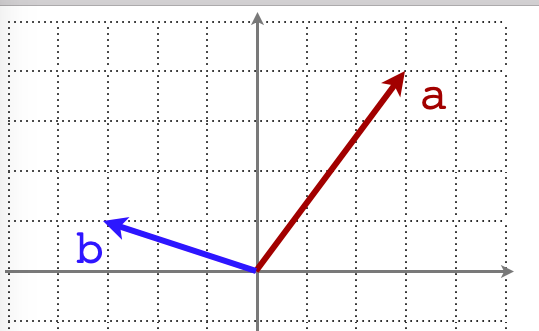
\includegraphics [scale=0.4] {basic_vectors.png} \end{center}

Vectors are written in bold type:
\[ \mathbf{a} = \langle \ 3 , 4 \ \rangle \]
\[ \mathbf{b} = \langle \ -3 , 1 \ \rangle \]

A vector has one property of a line, slope, but the fixed magnitude means that a vector does not extend to infinity as a line does.  The squared length of a vector can be computed as the sum of the squares of its components, according to Pythagoras.
\[ ( \text{length }\mathbf{a})^2 = |\mathbf{a}|^2 = 3^2 + 4^2 \]

By convention, we allow vectors to move about in space.  We mean that two vectors of the same length, and pointing in the same direction are considered to be the same object, regardless of where they are located in space.  (Some physics problems don't allow this, but in math it's the usual case).  

So if we have the vector $\mathbf{v} = \langle \ 1,1 \ \rangle$ starting at the origin $(0,0)$ and ending at the point $(1,1)$, and compare it to a second vector $\mathbf{u}$ that starts from $(2,0)$ and ends at $(3,1)$, those are considered to be the same vector.

As you might guess, the vector that connects two points $(x_1,y_1)$ and $(x_2,y_2)$  is 
\[ \mathbf{p} = \ \langle \ x_2-x_1,y_2-y_1 \rangle \  \] 
If we do the subtraction in reverse we have 
\[ \mathbf{q} = \  \langle \ x_1-x_2,y_1-y_2 \rangle \  \]
\[ \mathbf{p} = - \mathbf{q} \]

Vectors add by adding their components:
\[ \mathbf{a} = \langle \ 3 , 4 \ \rangle \]
\[ \mathbf{b} = \langle \ -3 , 1 \ \rangle \]
\[ \mathbf{a} + \mathbf{b} = \langle \ 0 , 5 \ \rangle \]
Subtraction works the same way.

From a linear algebra point of view, a vector is simply an ordered collection of numbers
\[  \mathbf{u} =  \ \langle \ u_1, u_2, \cdots \ u_n \rangle \  \]
where $n$ could be very large, even infinite.  

However, a lot of work is done in two or three dimensions (officially $\mathbb{R}^2$ and $\mathbb{R}^3$), and the principles developed there carry over nicely into $n$-dimensional space.  So let's start by thinking about a two-dimensional vector

\[ \mathbf{u} =  \ \langle \ u_1, u_2 \ \rangle \  \]

As I've said, the vector $\mathbf{u}$ can be thought of as an arrow that goes from the origin to the point $(u_1,u_2)$.  It has both length and direction, with the length given by
\[ |\mathbf{u} | = \sqrt{u_1^2 + u_2^2} \]

and its direction is
\[ \frac{u_2}{u_1} = \tan \ \theta, \ \ \ \  \theta = \tan^{-1} \ \frac{u_2}{u_1} \]
where $\theta$ is the angle the vector makes (rotating counter-clockwise) from the positive x-axis.

Any vector can be converted into a \emph{unit vector}, a vector of length one, by dividing by its length.  For example if $\mathbf{u} =\ \langle \ 1,2 \ \rangle$ then 

\[ \hat{\mathbf{u}} =  \frac{1}{|\mathbf{u}|}\ \mathbf{u} = \ \langle \ \frac{1}{\sqrt{5}}, \frac{2}{\sqrt{5}} \rangle \ \]
$\hat{\mathbf{u}}$ is a unit vector pointing in the same direction as $\mathbf{u}$.

The line through the origin with slope $m = u_2/u_1$ and equation
\[ y = mx \] 
can be thought of as the extension of vector $\mathbf{u}$ obtained by multiplying some $t$ times $\mathbf{u}$ for all $t \in \mathbb{R}$.  We have stretched the vector to infinity, and beyond!

The standard unit vectors point in the direction of the $x$, $y$ and $z$ axes.
\[ \hat{\mathbf{i}} = \ \langle \ 1, 0, 0 \ \rangle \]
\[ \hat{\mathbf{j}} = \ \langle \ 0, 1, 0 \ \rangle \]
\[ \hat{\mathbf{k}} = \ \langle \ 0, 0, 1 \ \rangle \]

We can write the vector using these unit vectors as
\[ \mathbf{a} = \langle \ 3 , 4 \ \rangle = 3 \cdot \hat{\mathbf{i}} + 4 \cdot \hat{\mathbf{j}}  \]

\section*{Dot product}
We now introduce a procedure for multiplying two vectors, the \emph{dot product}, and derive the relationship between the dot product of two vectors and the angle between them.  Suppose we have two vectors
\[ \mathbf{a} = \ \langle a_1,a_2 \rangle \]
\[ \mathbf{b} = \ \langle b_1,b_2 \rangle \]

Geometrically, we might think of these as being one vector extending from the origin in the $x,y$-plane to the point $(a_1,a_2)$, and the other vector extending from the origin to $(b_1,b_2)$.  The dot product is defined as 
\[ \mathbf{a} \cdot \mathbf{b} = a_1 b_1 + a_2 b_2 \]

We can extend this to a pair of vectors in $n$-dimensional space
\[ \mathbf{a} = \ \langle a_1,a_2, \dots a_n \rangle \]
\[ \mathbf{b} = \ \langle b_1,b_2, \dots b_n \rangle \]
\[ \mathbf{a} \cdot \mathbf{b} = a_1 b_1 + a_2 b_2 + \dots + a_n b_n = \sum_{i=0}^{n} a_i b_i \]

The two vectors being multiplied (whose dot product is computed) must have the same dimension, the same $n$.  Also, the result of the multiplication---the dot product---is a number.  This is in contrast to another form of vector multiplication (the cross-product) which yields a vector as the result.

\subsection*{notation}

The dot ($\cdot$) in the dot product may also used to set apart two multiplicands in scalar multiplication, to increase clarity.  So, you ask, how can we tell what is meant?  Well, consider
\[ v \cdot \frac{1}{v} \]
\[ \mathbf{a} \cdot \mathbf{b} \]
It's a dot product if the two objects are vectors, otherwise it's multiplication.

\subsection*{Some properties}
The dot product obeys the usual rules:  it is associative, commutative and distributive.  

The commutative property of the dot product:
\[ \mathbf{a} \cdot \mathbf{b} =  \mathbf{b} \cdot \mathbf{a} \]
follows from the same property for multiplication of real numbers, since
\[ \mathbf{a} \cdot \mathbf{b} = \sum_{n} a_n b_n \]
\[ =  \sum_{n} b_n a_n =  \mathbf{b} \cdot \mathbf{a} \]

For the distributive property, suppose
\[ \mathbf{b} = \mathbf{c} + \mathbf{d} \]
Then 
\[  \mathbf{a} \cdot \mathbf{b} =  \mathbf{a} \cdot ( \mathbf{c} + \mathbf{d}) = \mathbf{a} \cdot \mathbf{c} + \mathbf{a} \cdot \mathbf{d} \]

You can easily verify this by computing each term of the respective products.
\[ \mathbf{b} = \ \langle b_1,b_2 \rangle \ = \mathbf{c} + \mathbf{d} = \ \langle c_1+d_1,c_2+d_2 \rangle \ \]  
\[  \mathbf{a} \cdot \mathbf{b} = a_1(c_1 + d_1) + a_2(c_2+d_2) \]  
\[ =  a_1 c_1 + a_1 d_1 + a_2 c_2 + a_2 d_2  \]
\[ =  a_1 c_1 + a_2 c_2 + a_1 d_1 + a_2 d_2  \]
\[ = \mathbf{a} \cdot \mathbf{c} + \mathbf{a} \cdot \mathbf{d} \]

Another example that we will need below is
\[ ( \mathbf{a} -  \mathbf{b}) \cdot ( \mathbf{a} -  \mathbf{b}) =  \mathbf{a} \cdot \mathbf{a} -  \mathbf{a} \cdot \mathbf{b} -  \mathbf{b} \cdot \mathbf{a} +  \mathbf{b} \cdot \mathbf{b}   \]
by the commutative property
\[ =  \mathbf{a} \cdot \mathbf{a} +  \mathbf{b} \cdot \mathbf{b}  - 2 \ \mathbf{a} \cdot \mathbf{b}  \]

\subsection*{Length of a vector}
As we said, the length of a vector $\mathbf{a} = \ \langle a_1,a_2 \rangle $, designated $|\mathbf{a}|$, is computed by a straightforward application of the Pythagorean Theorem:
\[ |\mathbf{a}|^2 = a_1^2 + a_2^2 \]
We leave the result as the square for simplicity.  

This is easily extended to more dimensions by sequential application of the same method.  
\begin{center} \includegraphics [scale=0.2] {vector_length.png} \end{center}

In $\mathbb{R}^3$:
\[ |\mathbf{a}|^2 = a_1^2 + a_2^2 + a_3^2 \]
In $\mathbb{R}^n$:
\[ |\mathbf{a}|^2 = a_1^2 + a_2^2 + \dots + a_n^2 \]
Notice that
\[ |\mathbf{a}|^2 = \mathbf{a} \cdot \mathbf{a} \]

\subsection*{Relation to $\theta$}
Now we are ready for the main idea.  Suppose we draw two vectors $\mathbf{a}$ and $\mathbf{b}$ in $\mathbb{R}^2$ with their tails at the same point.  Designate the angle between them as $\theta$ and the vector representing the side opposite as $\mathbf{c}$.  
\begin{center} 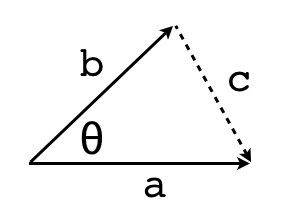
\includegraphics [scale=0.4] {dot1.png} \end{center}
The orientation of  $\mathbf{c}$ doesn't matter for the argument that follows.  As shown
\[ \mathbf{b} + \mathbf{c} = \mathbf{a} \]
\[ \mathbf{c} = \mathbf{a} - \mathbf{b} \]
Compute the dot product of $\mathbf{c}$ with itself
\[ \mathbf{c} \cdot \mathbf{c} = ( \mathbf{a} -  \mathbf{b}) \cdot ( \mathbf{a} -  \mathbf{b}) \]

Recalling the result from above, this is
\[ \mathbf{c} \cdot \mathbf{c} = \mathbf{a} \cdot \mathbf{a} +  \mathbf{b} \cdot \mathbf{b}  - 2 \ \mathbf{a} \cdot \mathbf{b}  \]
Since 
\[ |\mathbf{a}|^2 = \mathbf{a} \cdot \mathbf{a} \]
and so on, we have that
\[ \mathbf{c} \cdot \mathbf{c} =  \mathbf{a} \cdot \mathbf{a} +  \mathbf{b} \cdot \mathbf{b}  - 2 \ \mathbf{a} \cdot \mathbf{b}  \]
\[ |\mathbf{c}|^2 =  |\mathbf{a}|^2 + |\mathbf{b}|^2  - 2  \ \mathbf{a} \cdot \mathbf{b}  \]

Does this remind you of the \hyperref[sec:Law_of_cosines]{\textbf{law of cosines}}?

\[ c^2 = a^2 + b^2 - 2ab \cos \theta \]

Comparing the two equations, we see that
\[ \mathbf{a} \cdot \mathbf{b} = |\mathbf{a}| \ |\mathbf{b}| \ \cos \theta \]
This relationship is extremely useful because it allows us to compute the cosine of the included angle via the dot product.  

Even more important, two vectors which are perpendicular will have $\cos \theta = 0$, so their dot product is zero.  Two vectors in pointed in the same direction have $\cos \theta = 1$ so it's just the product of the magnitudes.

This result extends to vectors in $\mathbb{R}^n$.  Proof:  choose a coordinate system where the two vectors lie in the same plane.  Then apply the standard method.

For example, suppose I have the vector
\[ \mathbf{u} = \ \langle p,q \rangle \]
Find a vector $\mathbf{v}$ perpendicular to $\mathbf{u}$.
\[ \mathbf{v} = \ \langle q,-p \rangle \ \]
$\mathbf{v}$ is perpendicular to $\mathbf{u}$ because
\[ \mathbf{u} \cdot \mathbf{v} = pq + q(-p) = 0 \]

How to find a vector in $\mathbb{R}^5$ perpendicular to $\langle 1,1,1,1,0 \rangle$?
Any vector of the form $\langle 0,0,0,0,k \rangle $ will do, where k is some real number.

\subsection*{Alternate derivation}
Here is another approach which doesn't depend on knowing the law of cosines, but uses the addition rule for cosine instead.

\begin{center} 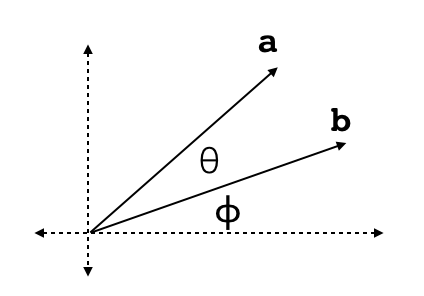
\includegraphics [scale=0.4] {dot4.png} \end{center}

Vector $\mathbf{a}$ forms an angle $\theta$ with vector $\mathbf{b}$. $\mathbf{b}$ forms an angle $\phi$ with the $x$-axis, so the angle between $\mathbf{a}$ and the $x$-axis is $\theta + \phi$.

Find the dot product using components.  If $a = |\mathbf{a}|$ and $b = |\mathbf{b}|$ then
\[ a_x = a \cos ( \theta + \phi ) \]
\[ b_x = b \cos \phi \]
\[ a_y = a \sin ( \theta + \phi ) \]
\[ b_y = b \sin \phi \]
So
\[ \mathbf{a} \cdot \mathbf{b} = a_x b_x + a_y b_y \]
\[ = ab \ [ \ \cos (\theta + \phi ) \cos \phi + \sin  (\theta + \phi ) \sin \phi \ ] \]

Using the rule
\[ \cos s - t = \cos s \cos t + \sin s \sin t \]
the part in parentheses is
\[ \cos (\theta + \phi ) \cos \phi + \sin  (\theta + \phi ) \sin \phi \]
\[ = \cos (\theta + \phi - \phi) = \cos \theta \]

Another important property is that the value of the dot product is \emph{independent} of the coordinate system chosen, because rotation or translation cannot change the lengths of the vectors nor the angle between them.

\subsection*{Projection}
If $|\mathbf{a}| = 1$ we say that $\mathbf{a}$ is a \emph{unit vector}.  In that case
\[ \mathbf{b} \cdot \mathbf{a} = |\mathbf{b}| \cos \theta \]
Looking at the figure, $|\mathbf{b}| \cos \theta$ is the length of the \emph{projection} of $\mathbf{b}$ on $\mathbf{a}$.  (Recall that the dot product is a scalar---a number---and not a vector).
\begin{center} 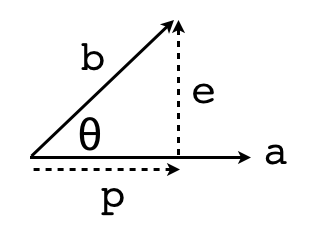
\includegraphics [scale=0.4] {dot3.png} \end{center}
The result, $\mathbf{b} \cdot \mathbf{a} = |\mathbf{b}| \cos \theta$, is the length of the part of $\mathbf{b}$ that extends in the same direction as $\mathbf{a}$.  The corresponding vector is 
\[ \mathbf{p} = (\mathbf{b} \cdot \mathbf{a}) \ \mathbf{a} \]
The other component of $\mathbf{b}$ is the part that is perpendicular to $\mathbf{p}$
\[ \mathbf{p} + \mathbf{e} = \mathbf{b} \]
We compute $\mathbf{e}$ as the difference $\mathbf{b} -  \mathbf{p}$.  $\mathbf{e}$ is the part of $\mathbf{b}$ that is perpendicular to the projection.  As a final note, the formula given here is a simplification for the situation in which $\mathbf{a}$ is a unit vector.  If not, the complete formula is:
\[ \mathbf{p} = \frac{\mathbf{b} \cdot \mathbf{a}}{\mathbf{a} \cdot \mathbf{a}} \ \mathbf{a} \]

Vectors allow simple proofs for some geometric theorems such as Ceva's theorem and the law of cosines.

\subsection*{example}

Here is a problem from Nahin:
\begin{center} 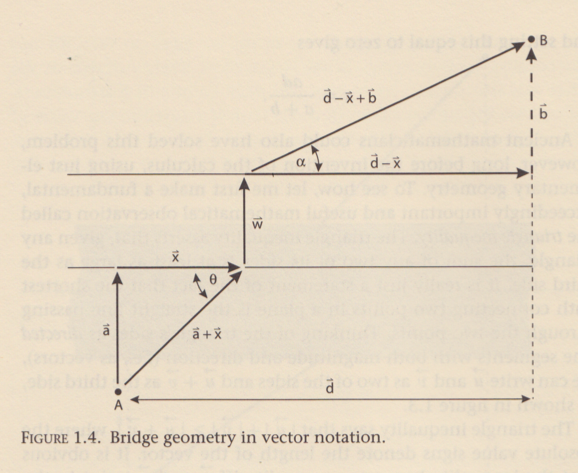
\includegraphics [scale=0.5] {bridge_geometry.png} \end{center}

Two towns are on opposite sides of a river at points $A$ and $B$.  It is desired to choose the site of a bridge so as to minimize the distance between the two towns when traveling over the bridge.  The problem can be set up algebraically and solved by differential calculus.  However, the vector approach is more fun, and allows us to introduce the important \emph{triangle inequality}.

Vectors are shown in the figure:  $\mathbf{a}$ is the perpendicular distance from $A$ to the river, and similarly for $\mathbf{b}$.  $\mathbf{x}$ determines the placement of the bridge.  If the horizontal distance between $A$ and $B$ is $\mathbf{d}$, then $\mathbf{d} - \mathbf{x}$ is the horizontal distance between $B$ and the bridge.  The distance across the bridge is $\mathbf{w}$, which cannot be changed.  Its length will just be added onto our shortest path.

We want to choose $\mathbf{x}$ so that the path from $A$ to $B$ is the shortest.  The path from $A$ to the bridge is $\mathbf{a} + \mathbf{x}$, that from the bridge to $B$ is $\mathbf{b} + \mathbf{d} -  \mathbf{x}$ so all together we have (taking the lengths of the vectors)
\[ L = |\mathbf{a} + \mathbf{x}| + |\mathbf{b} + \mathbf{d} -  \mathbf{x}| \]

The triangle inequality says that the lengths of two sides of a triangle add to be larger than or equal to the length of the third side.
\begin{center} 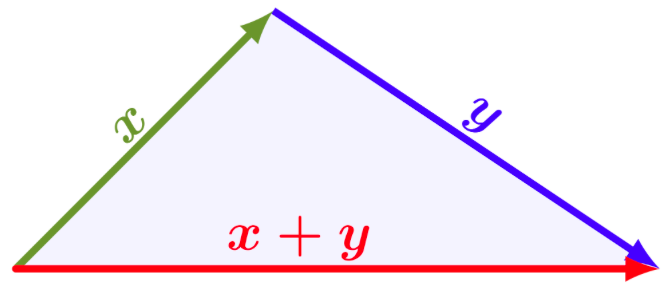
\includegraphics [scale=0.3] {triangle_inequality.png} \end{center}
\[ |\mathbf{x}| + |\mathbf{y}| \ge |\mathbf{x} + \mathbf{y}| \]

The rule is that the minimal value for the sum $|\mathbf{x}| + |\mathbf{y}|$ occurs when they point in the same direction.

In our problem, the minimum length occurs when $\mathbf{a} + \mathbf{x}$ and $\mathbf{b} + \mathbf{d} -  \mathbf{x}$ point in the same direction.  In other words, when $\theta = \alpha$.  

Then, by similar triangles,
\[ \frac{x}{a} = \frac{d-x}{b} \]
\[ bx = ad - ax \]
\[ x = \frac{ad}{a + b} \]

\subsection*{example}

Here is one from Strang.
\begin{center} 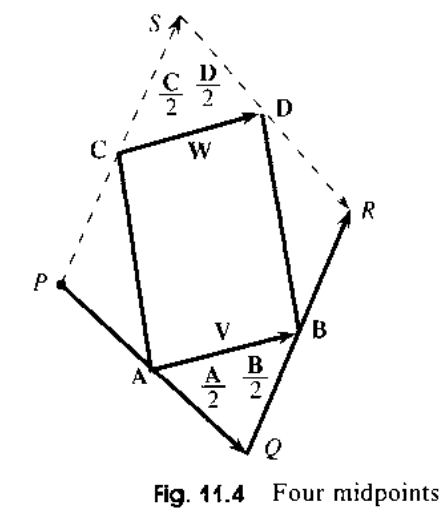
\includegraphics [scale=0.5] {midpoint_vectors.png} \end{center}
Consider \emph{any} four-sided figure in space, such as $PQRS$ in the figure.  (Note:  $|\mathbf{A}| \ne |\mathbf{B}|$, and so on, and $S$ is not co-planar with $P,Q,R$.  I claim that the midpoints of the sides form a parallelogram $ABCD$.

We will prove that $\mathbf{V} = \mathbf{W}$.

The figure makes it almost obvious.
\[ \mathbf{V} = \frac{\mathbf{A}}{2} + \frac{\mathbf{B}}{2} \]
\[ \mathbf{W} = \frac{\mathbf{C}}{2} + \frac{\mathbf{D}}{2} \]
The segment from $P$ to $R$ can be covered in two ways
\[ \mathbf{A} + \mathbf{B} = \mathbf{C} + \mathbf{D} \]
Divide both sides by $2$ and obtain
\[ \frac{\mathbf{A}}{2} + \frac{\mathbf{B}}{2}  = \frac{\mathbf{C}}{2} + \frac{\mathbf{D}}{2} \]
\[ \mathbf{V} = \mathbf{W} \]
$\square$

\subsection*{example}

And here is one from Euclid:
\begin{center} 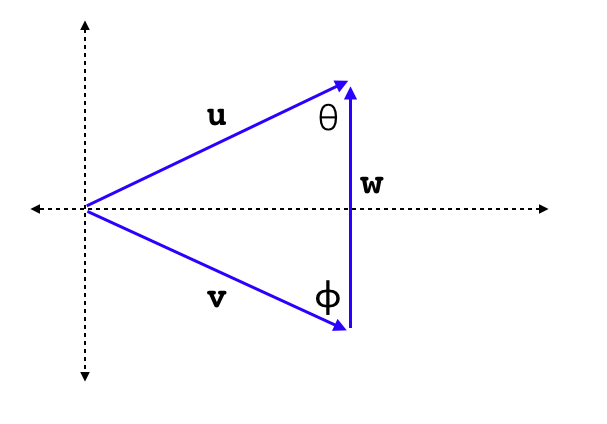
\includegraphics [scale=0.4] {isosceles2.png} \end{center}
We are given a triangle with two sides the same length (isosceles).  Without loss of generality, draw the triangle with its vertex at the origin and the midpoint of the third side on the $x$-axis.

To prove:  $\theta = \phi$.

Let
\[ \mathbf{u} = \ \langle a, b \rangle \]
\[ \mathbf{v} = \ \langle a, -b \rangle \]
\[ \mathbf{w} = \ \langle 0, 2b \rangle \]

We compute the dot products so that the angle between the vectors is acute and the dot product is $> 0$.
\[ \mathbf{u} \cdot \mathbf{w} = 2b^2 \]
\[ = |\mathbf{u}| |\mathbf{w}| \cos \theta =  \sqrt{a^2 + b^2} \ 2b \cos \theta \]
\[ \cos \theta = \frac{b}{\sqrt{a^2 + b^2}} \]
which is also obvious from the figure.  We didn't need vectors for this.

\[ (- \mathbf{w}) \cdot \mathbf{v} = 2b^2 \]
\[ = \sqrt{a^2 + b^2} \ 2b \cos \phi \]
\[ \cos \phi = \frac{b}{\sqrt{a^2 + b^2}} \]

We obtain the same result for $\cos \phi$ as for $\cos \theta$ and then finally
\[ \theta = \phi \]

\end{document}